\subsection{Evaluation}
\begin{figure}[t]
	\begin{center}
		\fbox{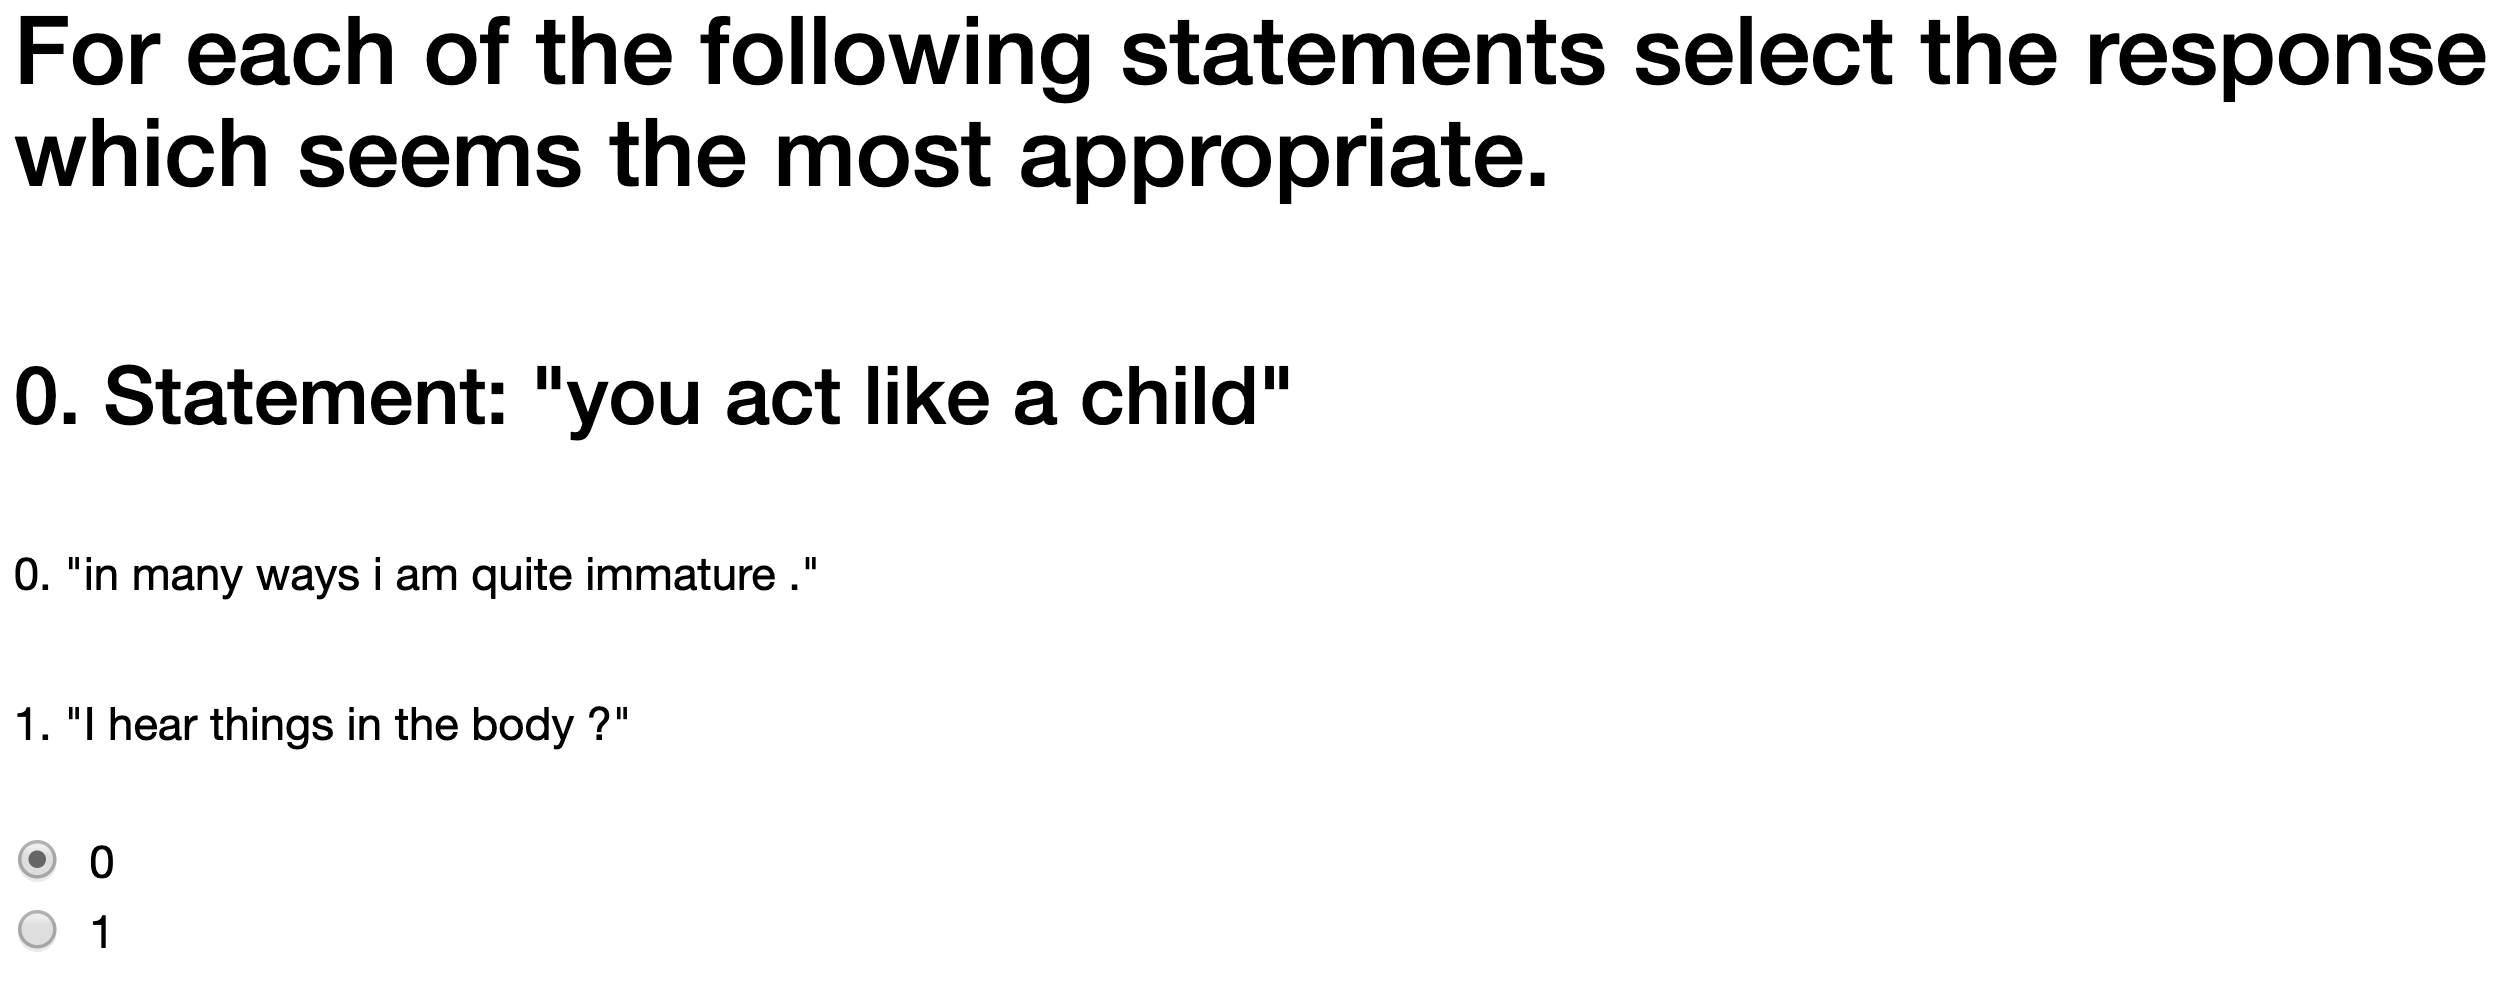
\includegraphics[width=\textwidth]{QuestionExample.PNG}}
	\end{center}
	\caption{Example of a question for the human evaluation metric.}
	\label{fig:human_eval_question}
\end{figure}
To evaluate the performance of our models we considered two types of metrics: a collection of automatic metrics and a human metric.
%For testing, we reserved $20\%$ of each datatset.
%These test sets were sampled at random from the raw dataset.
%As we will discuss later, we report both types of metric for each model and each test set independently.

The automatic metrics we considered were bilingual evaluation understudy (BLEU), recall-oriented understudy for gisting evaluation (ROUGE), metric for evaluation of translation with explicit ordering (METEOR) and word error rate (WER) \cite{Papineni:2002:BMA:1073083.1073135, lin-2004-rouge, denkowski:lavie:meteor-wmt:2014}.
These metrics are often used to evaluate the performance of translation bots and in some cases other chatbots.
However, despite a strong relationship between chatbots with personality and translation bots, these metrics are believed to be poor measures of performance for personality chatbots \cite{Radz2017, Xing2018, LiuLSNCP16, SerbanLCP15}.
Despite this, they are still often used to evaluate some aspects of a chatbot's performance.

The idea behind each of these metrics is to compared a response generated by one of our models against a saved test response.
The general idea behind BLEU, ROUGE and METEOR is to measure the overlap of words in the generated response and the test response.
The BLEU score is the normal BLEU score computed with weights $(.25,.25,.25,.25)$.
For ROUGE we report the  F1 score computed after calculating both the precision and recall.
We consider both ROUGE-1 and ROUGE-$\ell$.
We also collected additional ROUGE scores (e.g. ROUGE-$4$) but they were approximately $0$ for all of our experiments.
%A powerful tool for the METEOR metric is that it uses synonyms from a stored synonym library to extend this from exact word overlap to the overlap of closely related words.
We report the normal METEOR score.
All of these metrics output a score between $0$ and $1$ with $1$ being the best.
The WER metric computes the word edit distance between the generated response and the test response and outputs this divided by the length of the test response. 
For the WER score, a small number was best but the numbers could range to be arbitrarily large (if the generated response was very large compared to the test response).
We then average these scores over our entire dataset except for ROUGE which uses a corpus calculation.
We refer the reader to the appropriate references for a detailed explanation of these metrics.

For the human based evaluation we designed a jupyter notebook which randomly generated questions for each model from each dataset.
Each question had a test statement, test response and generated response.
The responses were placed in random order so that the tester would not know which was the generated response.
The tester was asked to select which response was most Joey like or appropriate for Joey to say given the response (See Figure \ref{fig:human_eval_question}).
We considered 4 testers familiar with Friends and the Joey character. 
Each tester answered at least 30 of these questions for each model and dataset combination.
For each tester and each combination, we calculated a final score by taking the total fraction of questions where the generated response was selected.
We then averaged them to get our final score for the combination.
Like the classic Turing test, an ideal outcome would be a score of $.50$.
That is, our model would create responses as Joey like as those from the actual show and the user would ultimately have to randomly pick between.


